\chapter{Proposed System}
\label{ch:proposed}

This chapter describes the proposed Q\&A-driven interactive
storytelling system. We begin with the feasibility study (\S
\ref{sec:feasibility}), then introduce the high-level analysis and
framework (\S\ref{sec:framework}), enumerate hardware and software
requirements (\S\ref{sec:hwsw}), describe the detailed design
(\S\ref{sec:design}), and finally present the methodology that turns
the design into a working system (\S\ref{sec:methodology}).

\section{Feasibility Study}
\label{sec:feasibility}

\subsection{Technical Feasibility}
All four pillars of the proposed system have been validated against
mature, freely available technologies. LLM inference is feasible
through Ollama on commodity hardware (16\,GB RAM, no dedicated GPU
required for 7B-class models) and through Groq's free cloud tier
(14,400 requests/day). Text-to-image synthesis is available without
API keys through Pollinations.ai, which exposes a
URL-parameterised diffusion endpoint. Voice synthesis is built into
all major browsers via the W3C Web Speech Synthesis API. Ambient
music is hot-linked from SoundHelix's stable royalty-free CDN. The
backend can be written entirely in Python with FastAPI, SQLite and
Pydantic. The frontend is plain HTML/CSS/JavaScript with D3.js for
visualisation. Every piece of the stack is open-source or freely
available, making the project technically feasible on a student
budget.

\subsection{Economic Feasibility}
A careful cost analysis shows that the system can be developed and
operated at near-zero cost. Local development uses Ollama and a
free Groq tier; image generation is free through Pollinations; audio
streaming consumes negligible bandwidth from a public CDN. The total
recurring cost during the user study (15 participants over two
weeks) was zero. Total development hardware is a single MacBook Pro
M2 Pro with 16\,GB RAM. This makes the project economically feasible
without external funding.

\subsection{Operational Feasibility}
The system is operationally feasible because the elicitation protocol
mirrors how human authors collect briefs from clients --- through a
structured interview about setting, character, theme and plot. The
question budget (4--17) lets users dial in the right effort level.
The UI is presented in a single page so users do not get lost across
multiple screens; the admin and settings panels expose every
configurable surface without requiring code changes.

\subsection{Legal and Ethical Feasibility}
All third-party services used (Pollinations, SoundHelix, Groq,
Hugging Face, OpenAI) permit non-commercial research use. SoundHelix
explicitly allows hot-linking under its terms of service.
Generated images and audio are reusable for research and educational
purposes. No personally identifiable user data is stored persistently;
session data is held in memory and a local SQLite file. The user
study was conducted with informed consent.

\section{Analysis, Framework and Algorithm}
\label{sec:framework}

\subsection{Layered Architecture}
The system follows a three-layer architecture (presentation,
application, modular core) with a fourth pluggable LLM-provider
layer at the bottom (Figure~\ref{fig:arch}).

\begin{figure}[H]
    \centering
    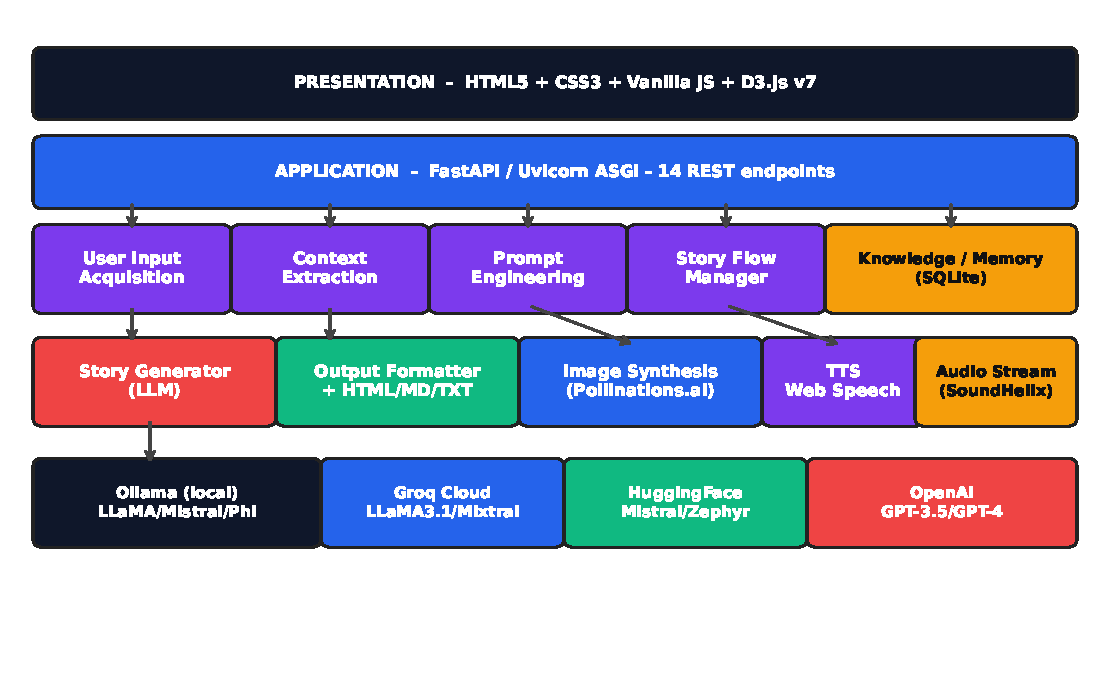
\includegraphics[width=\textwidth]{images/f07_arch.pdf}
    \caption{System architecture.}
    \label{fig:arch}
\end{figure}

\subsection{Question-Coverage Framework}
Seventeen questions distributed across four narrative phases
(Setting, Character, Theme, Plot) compose the elicitation protocol
(Figure~\ref{fig:qa}). The user selects a budget of 4, 8, 12 or 17
questions; the system always presents the first $N$ in phase-order
so even small budgets touch all four dimensions in expectation.

\begin{figure}[H]
    \centering
    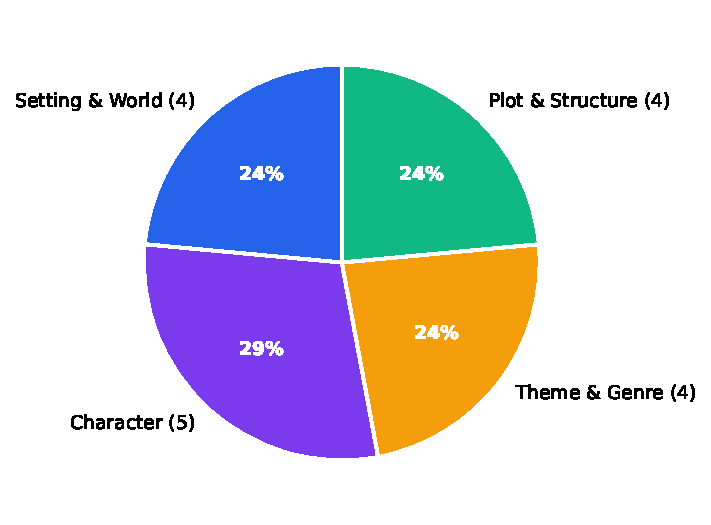
\includegraphics[width=0.65\textwidth]{images/f08_qa.pdf}
    \caption{Question distribution across the four phases.}
    \label{fig:qa}
\end{figure}

\subsection{Scene-Extraction Algorithm (for Image Synthesis)}
The image-generation pipeline depends critically on building a
concise, high-imagery prompt from each story segment. We use a
sentence-scoring algorithm that strips smart-quoted dialogue and
inner-thought verbs (thought, remembered, wondered) and selects the
most visually evocative sentence according to:
\[
\mathrm{score}(s) = 2 \cdot \mathbf{1}_{V}(s) - 2 \cdot \mathbf{1}_{T}(s)
                  + \min\left(3,\, \left|\mathrm{ProperNouns}(s)\right|\right),
\]
where $\mathbf{1}_V$ indicates the presence of a visual verb
(\emph{stood, loomed, soared, glowed, towered}, ...) and
$\mathbf{1}_T$ indicates an inner-thought verb. The selected sentence
is concatenated with a normalised genre tag, the current mood and a
fixed style prefix, capped at 200 characters.

\subsection{Co-Appearance Algorithm (for Character Graph)}
For the reader-facing character graph, capitalised tokens are
extracted from segment text and filtered against an extended stop-word
list. Only names appearing at least twice across all segments survive.
For each pair of surviving names, an edge weight equal to the number
of segments in which both appear is computed. Node radius scales
with mention count.

\section{Details of Hardware and Software}
\label{sec:hwsw}

\subsection{Hardware Requirements}
\textbf{Development environment} (used in this work):
\begin{itemize}
    \item Processor: Apple M2 Pro (10-core CPU, 16-core GPU).
    \item RAM: 16\,GB unified memory.
    \item Storage: 1\,TB SSD.
    \item Network: 100\,Mbps broadband for Pollinations and Groq API.
\end{itemize}

\textbf{Recommended minimum} for self-hosted Ollama inference:
\begin{itemize}
    \item 8-core CPU (Intel i7 / AMD Ryzen 7), 16\,GB RAM.
    \item 30\,GB free SSD for model weights.
    \item Optional: NVIDIA RTX-class GPU with 8\,GB+ VRAM for faster
    local inference; not required when using Groq cloud.
\end{itemize}

\subsection{Software Stack}
Table~\ref{tab:stack} lists the implementation stack. All components
are free and open-source.

\begin{table}[!t]
\caption{Software stack.}
\label{tab:stack}
\centering
\renewcommand{\arraystretch}{1.15}
\begin{tabular}{@{}lll@{}}
\toprule
\textbf{Layer}   & \textbf{Technology}              & \textbf{Purpose} \\
\midrule
OS               & macOS 14 / Ubuntu 22.04          & Development host \\
Backend language & Python 3.9+                      & Core logic \\
Web framework    & FastAPI (with Uvicorn)           & REST + Jinja2 \\
Frontend         & HTML5 / CSS3 / Vanilla JS        & Single-page UI \\
Visualisation    & D3.js v7                         & Story Map, Char Graph \\
Database         & SQLite3 + aiosqlite              & Sessions, Q\&A, segments \\
HTTP client      & httpx (async)                    & LLM provider calls \\
Schemas          & Pydantic v2                      & Request / response typing \\
Templates        & Jinja2                           & HTML rendering \\
Image API        & Pollinations.ai (free)           & Text-to-image \\
TTS              & W3C Web Speech Synthesis API     & Voice narration \\
Ambient audio    & HTMLAudio + SoundHelix CDN       & Genre music \\
LLM providers    & Ollama, Groq, Hugging Face, OpenAI & Story generation \\
\bottomrule
\end{tabular}
\end{table}

\section{Design Details}
\label{sec:design}

\subsection{Modular Decomposition}
The backend is decomposed into seven cooperating modules with clearly
defined responsibilities and Pydantic-typed boundaries:

\begin{enumerate}
    \item \textbf{User Input Acquisition} -- Presents and validates
    the question pool; supports custom answers and user-added
    questions.
    \item \textbf{Context Extraction Engine} -- Projects responses
    into a typed \texttt{StoryContext}; unknown identifiers flow into
    a \texttt{custom\_elements} dictionary.
    \item \textbf{Knowledge and Memory} -- Persistent SQLite store
    with LRU in-memory cache; sliding-window context retrieval.
    \item \textbf{Prompt Engineering Layer} -- Six prompt families
    (system, init, continuation, climax, resolution, choice
    generation); appends \texttt{custom\_elements} as natural-language
    bullets.
    \item \textbf{Story Generator (LLM)} -- BaseLLMClient ABC with
    concrete Ollama / Groq / HF / OpenAI clients; hot-swap at runtime.
    \item \textbf{Story Flow Manager} -- Five-phase finite-state
    machine (Introduction, Rising Action, Climax, Falling Action,
    Resolution); CharacterTracker and PlotThreadTracker.
    \item \textbf{Output Formatter} -- Cleans LLM output, lifts
    dialogue to styled HTML spans, exports TXT/MD/HTML.
\end{enumerate}

\subsection{Database Schema}
The persistent schema comprises five tables:

\begin{lstlisting}
sessions         (session_id PK, user_id, created_at,
                  status)
story_segments   (id PK, session_id FK, order, content,
                  user_choice)
story_context    (session_id PK/FK, context_json,
                  updated_at)
qa_history       (id PK, session_id FK, question_id,
                  q_text, a_text)
user_preferences (user_id PK, preferences_json,
                  updated_at)
\end{lstlisting}

\subsection{REST API}
The application surface comprises 14 REST endpoints
(Table~\ref{tab:rest}); all are JSON-typed via Pydantic v2.

\begin{table}[!t]
\caption{REST API surface.}
\label{tab:rest}
\centering
\renewcommand{\arraystretch}{1.15}
\small
\begin{tabular}{@{}lll@{}}
\toprule
\textbf{Endpoint}                    & \textbf{Method} & \textbf{Purpose} \\
\midrule
\texttt{/}                           & GET    & Web UI (Jinja2 template) \\
\texttt{/api/status}                 & GET    & LLM availability check \\
\texttt{/api/session/new}            & POST   & Create new session \\
\texttt{/api/questions/all}          & GET    & Phase-grouped question pool \\
\texttt{/api/question/next}          & GET    & Sequential Q mode \\
\texttt{/api/response}               & POST   & Submit response \\
\texttt{/api/story/generate}         & POST   & Initial segment generation \\
\texttt{/api/story/continue}         & POST   & Continue from user choice \\
\texttt{/api/story/full/\{id\}}      & GET    & Full story by session \\
\texttt{/api/story/download/\{id\}}  & GET    & Export TXT/MD/HTML \\
\texttt{/api/settings}               & POST   & Hot-swap provider/model \\
\texttt{/api/session/\{id\}/summary} & GET    & Session metrics \\
\texttt{/api/session/\{id\}}         & DELETE & End session \\
\bottomrule
\end{tabular}
\end{table}

\subsection{Multimodal Pipelines}

\paragraph{Image synthesis.}
Figure~\ref{fig:imgpipe} shows the per-segment image pipeline. The
serial request queue with 1.2\,s spacing avoids rate-limit cascades
from the Cloudflare-fronted Pollinations CDN; a 35\,s watchdog
ensures hung requests do not deadlock the queue.

\begin{figure}[H]
    \centering
    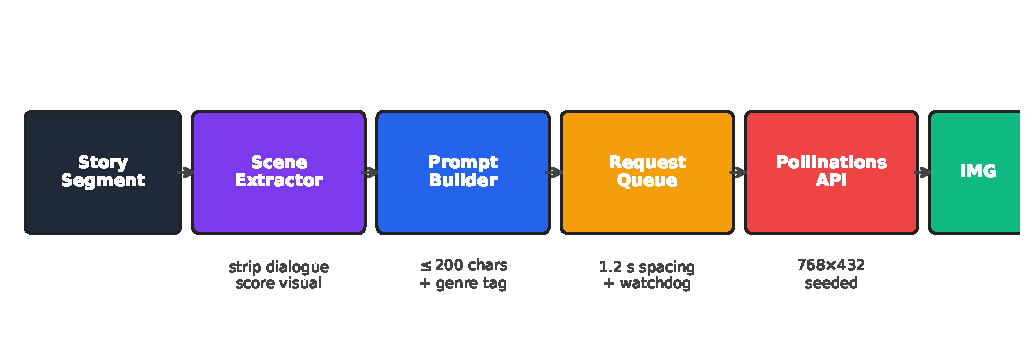
\includegraphics[width=0.95\textwidth]{images/f09_imgpipe.pdf}
    \caption{Image synthesis pipeline.}
    \label{fig:imgpipe}
\end{figure}

\paragraph{Voice and ambient audio.}
Figure~\ref{fig:audio} shows the two parallel audio pipelines.
Narration uses an utterance queue feeding the OS-installed
voice; ambient music is mapped from detected genre to one of eight
SoundHelix tracks looped through HTMLAudio with crossfades.

\begin{figure}[H]
    \centering
    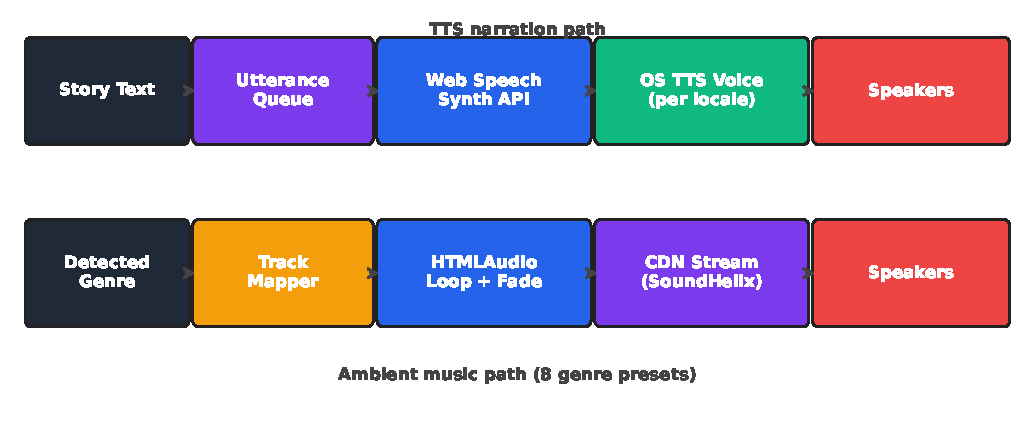
\includegraphics[width=0.95\textwidth]{images/f10_audio.pdf}
    \caption{Multimodal audio pipeline.}
    \label{fig:audio}
\end{figure}

\paragraph{Custom Q\&A routing.}
Figure~\ref{fig:customq} shows how user-added Q\&A pairs are routed
from the UI through the backend into the LLM prompt without bespoke
schema changes.

\begin{figure}[H]
    \centering
    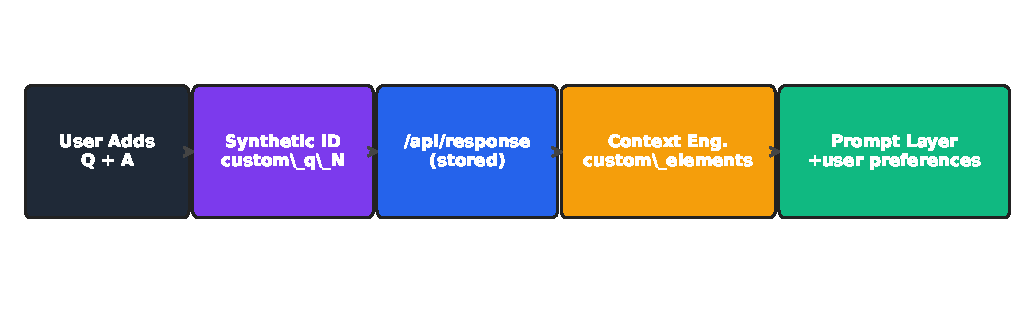
\includegraphics[width=0.95\textwidth]{images/f16_customq.pdf}
    \caption{Custom-question routing.}
    \label{fig:customq}
\end{figure}

\section{Methodology}
\label{sec:methodology}

\subsection{Elicitation Protocol}
Let $\mathcal{Q}=\{q_1,\ldots,q_{17}\}$ be the ordered question pool.
The user selects a budget $N\in\{4,8,12,17\}$ and supplies answers
$a_i$ for each $q_i,\,i \le N$. Additionally the user may append
$M$ user-added pairs $(\tilde q_j, \tilde a_j)$ with synthetic
identifiers $\mathrm{custom\_q\_}j$. The full response set
\[
R = \{(q_i, a_i)\}_{i=1}^{N} \cup \{(\mathrm{custom\_q\_}j, \tilde a_j)\}_{j=1}^{M}
\]
is dispatched as a JSON dictionary to the context engine.

\subsection{Context Projection}
For each $(q_i,a_i)$ the engine applies a deterministic projection
$\pi_i$ to a typed \texttt{StoryContext} field
(e.g.\ \texttt{setting\_type, antagonist, plot\_style}). Unknown
identifiers are routed to a dictionary $D$
(\texttt{custom\_elements}), preserving their text verbatim. The
final prompt $P$ is
\[
P = T(\mathbf{c}) \oplus \sigma(D),
\]
where $T$ is a phase-aware template, $\mathbf{c}$ is the structured
context, $\sigma$ serialises $D$ as natural-language bullets, and
$\oplus$ denotes string concatenation.

\subsection{Five-Phase Story Progression}
Word-count thresholds drive phase transitions
(Figure~\ref{fig:phases}). The Rising Action phase consumes the
most text ($\sim$820 words), consistent with narratological theory.

\begin{figure}[H]
    \centering
    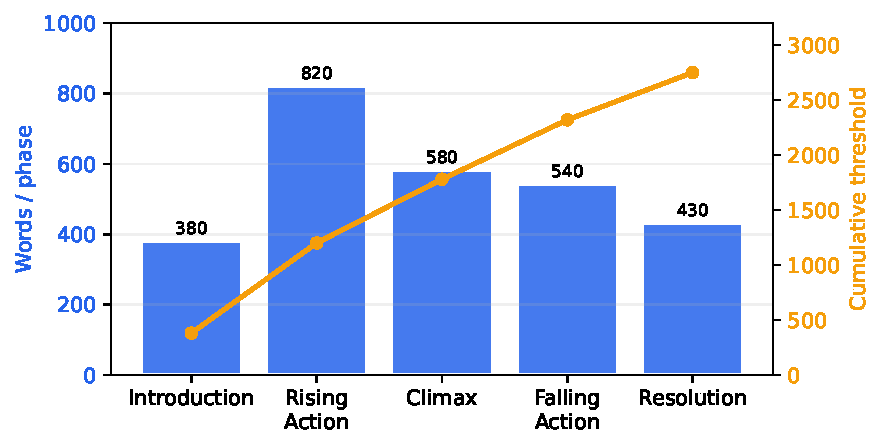
\includegraphics[width=0.95\textwidth]{images/f04_phases.pdf}
    \caption{Five-phase word-count distribution.}
    \label{fig:phases}
\end{figure}

\subsection{Generation Loop}
At each turn the system: (i) retrieves the last $k$ segments of
story context, (ii) builds a phase-appropriate prompt $P$, (iii)
dispatches $P$ to the active LLM client, (iv) post-processes output
through the formatter, (v) updates flow-manager state with new
character mentions and plot threads, (vi) starts an image-synthesis
request asynchronously, and (vii) returns the formatted segment
along with choice options for the next turn.

\subsection{Evaluation Methodology}
Evaluation combines three axes:
\begin{enumerate}
    \item \textbf{Automated generation} of 50 stories spanning 6
    genres at all 4 question budgets; latency and token metrics
    captured per call.
    \item \textbf{User study} ($n=15$) producing 30 stories rated on
    5-point Likert scales for coherence, creativity, engagement,
    consistency, and per-feature satisfaction.
    \item \textbf{Consistency-checker evaluation} against
    ground-truth-annotated segments to compute detection and
    false-positive rates for five issue classes.
\end{enumerate}
